% A talk.
%
% Beamer is a different kind of document: the unit is the frame rather than
% the page, and almost everything you would tune in an article is decided by
% the theme. Two rules survive from the article template: one idea per
% frame, and no sentence on a slide that you are also going to say out loud.

\documentclass[aspectratio=169]{beamer}

\usetheme{default}
\usecolortheme{seahorse}
\setbeamertemplate{navigation symbols}{}   % nobody has ever used these
\setbeamertemplate{footline}[frame number]

\usepackage[T1]{fontenc}
\usepackage{lmodern}
\usepackage{amsmath, amssymb}
\usepackage{graphicx}
\usepackage{booktabs}
\usepackage{siunitx}
\usepackage{tikz}

\usepackage[backend=biber, style=numeric, sorting=none]{biblatex}
\addbibresource{references.bib}

\title{A Working Title}
\subtitle{What this talk is actually about}
\author{Your Name}
\institute{Where you are}
\date{\today}

\begin{document}

\begin{frame}
  \titlepage
\end{frame}

\begin{frame}{What this is}
  \begin{itemize}
    \item One idea per frame.
    \item Three or four bullets at most, and none of them a paragraph.
    \item The slide is the evidence; the talk is the argument.
  \end{itemize}
\end{frame}

\begin{frame}{A result}
  \begin{columns}
    \begin{column}{0.5\textwidth}
      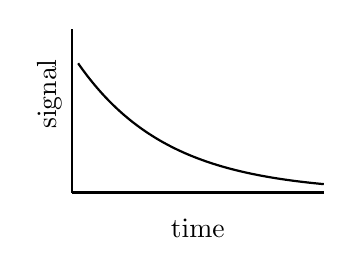
\begin{tikzpicture}[scale=0.8]
        \draw[thick] (0,0) -- (4,0) node[midway, below=6pt] {time};
        \draw[thick] (0,0) -- (0,2.6) node[midway, above=6pt, rotate=90] {signal};
        \draw[thick, smooth, domain=0.1:4, samples=60]
          plot (\x, {2.2 * exp(-0.7 * \x)});
      \end{tikzpicture}
    \end{column}
    \begin{column}{0.5\textwidth}
      The decay is exponential with a time constant of
      \SI{1.4}{\pico\second}, which is the one number in this talk worth
      remembering~\cite{knuth1984}.
    \end{column}
  \end{columns}
\end{frame}

\begin{frame}{What it means}
  \begin{itemize}
    \item What the result rules out.
    \item What it does not settle.
    \item What you would do next.
  \end{itemize}
\end{frame}

\end{document}
